\chapter{Architettura di una Applicazione Ibrida}
La scelta di seguire un determinato schema progettuale di una applicazione è stata fatta in base alle conoscenze apprese durante la mia esperienza di tirocinio in azienda, durante la quale non mi sono occupato dell'intera progettazione dell'applicazione, mi occupavo solo dello sviluppo \emph{frontend} di questa, ma per uno sviluppatore è necessario conoscere l'intera dinamica che si svolge all'interno di essa anche se non andrà a intervenire su determinate parti.\\

La politica che è stata intrapresa in azienda è stata quella della \emph{Separation of Concernes}(SoC), che in italiano si traduce in \emph{Separazione dei Compiti}. Si tratta di un principio di design dell'applicazione per dividere l'applicazione in sezioni distinte, e ad ogni sezione assegnare un particolare compito o risoluzione di un problema. Questa scelta progettuale introduce il concetto di \emph{modulo} di una applicazione, ovvero l'applicazione poi dipenderà dai moduli che andremo a creare e ad unire tra di loro. I moduli ragionevolmente saranno indipendenti uno dall'altro in modo tale da garantirne l'integrità e il loro re-utilizzo.\cite{wiki:soc}\\
In concetto appena visto astrae molto da una applicazione vera e propria, sta a chi la progetta decidere con che granularità  e se è veramente necessario applicarlo. Dato che parliamo di tecnologie web, un chiaro esempio si separazione dei compiti è quello della struttura di una pagina web, divisa in HTML per la struttura, CSS per lo stile, e Javascript per la logica e comportamento.\\

In questo capitolo andremo a vedere in che modo i compiti si possono separare all'interno di una applicazione web, per poi spostarci successivamente sul modello ibrido, in quanto eredità molti dei concetti che vedremo. Successivamente la trattazione proseguirà analizzando il ciclo di vita a cui si sottopongono le applicazioni in generale, in modo da poter poi illustrare nel capitolo successivo un esempio di sviluppo intrapreso in base ai dati e ai concetti forniti in questo. 
\section{Lo schema concettuale}
Nell'introduzione precedente si è detto che lo sviluppatore deve conoscere tutta la struttura della applicazione anche se ne andrà a sviluppare solo una parte. In questa sezione andremo a vedere lo \emph{schema concettuale} con il quale andremo a ad applicare la prima separazione dei compiti della nostra applicazione, ed i concetti correlati che possono servire.
\subsection{Frontend e Backend}
Queste due parole sono spesso usate in informatica in molti ambiti, nel contesto specifico dell'applicazione \texttt{frontend}(in italiano parte davanti) denota quella parte dell'applicazione responsabile di gestire l'interfaccia utente e i dati provenienti da essa, mentre \texttt{backend}(in italiano parte dietro) indica la sezione dell'applicazione dedita alla gestione dei dati provenienti dalla parte frontend. L'interazione che hanno le due parti è un chiaro esempio di interfaccia.\\
\textbf{Frontend:} questa è la parte caratteristica dell'applicazione, in quanto ne definisce il comportamento e l'aspetto, determinando la logica con cui si evolverà al rapporto con l'utente. A differenza della parte \emph{backend} questa non definisce nessuna manipolazione dei dati ma solo la loro rappresentazione(vista) determinando transizioni e/o animazioni.
Nella parte \emph{frontend} è inclusa anche la fase di definizione estetica dell'interfaccia, ma spesso questa spetta a una figura professionale distinta atta "vestire" l'applicazione.
\textbf{Backend:} questa parte è completamente diversa dalla prima, in quanto definisce la manipolazione dei dati all'interno dell'applicazione ma non da nessuna informazione caratteristica di essa. In particolare fornisce dei servizi ai quali la parte \emph{frontend} può accedere e recuperare/fornire dei dati, come ad esempio l'autenticazione di un utente a un servizio. Tutta la gestione dei dati che viene fatta da questa parte, viene oscurata alla parte \emph{frontend} per garantire un servizio di sicurezza molto elementare, in modo tale che se l'utente inserisce dei dati errati che vengono passati dalla parte \emph{frontend} a quella \emph{backend}, in modo errato, nessuna operazione verrà eseguita e l'integrità dei dati preservata.\\

A livello professionale molti sviluppatori si identificano appunto come \emph{frontend} e/o \emph{backend} developer per appunto identificarsi specializzati nello sviluppo di una parte specifica dell'applicazione.
Il vantaggio di usare un approccio di questo tipo sta nel fatto che la parte \emph{frontend} è l'unica specifica per una data applicazione. Se la parte \emph{backend} viene progettata bene, e possibile utilizzare i servizi che fornisce anche in futuro da altre applicazioni, pur seguendo il protocollo che richiede. Inoltre a livello professionale si può procedere parallelamente nello sviluppo delle parti in modo tale da ottimizzare i tempi, pur seguendo uno schema stabilito a priori.\\

Resta da spiegare come queste due parti comunichino tra di loro, il modo più elementare a cui verrebbe da pensare è sicuramente tramite dei messaggi. Quello di cui ci occuperemo successivamente è come vengono formati i messaggi e che protocollo di comunicazione devono rispettare.
\subsection{Pattern Client-Server}
\textbf{Definizione:} Il modello client-server è un modo per strutturare applicazioni distribuite che distingue due parti di un processo di comunicazione, la prima che fornisce una risorsa e/o un servizio chiamata server, la seconda che analogamente li può richiedere, chiamata client. La comunicazione in generale avviene attraverso la rete, ed è il client a iniziarla. Il compito del server è quello di predisporre le risorse che ha ai vari client che li chiedono, rimanendo appunto "in ascolto", il client invece non condivide le risorse con altri, può solo interagire con il server\cite{wiki:cliserv}.\\

Come si può già intuire le parti che verranno prese in questo modello saranno rispettivamente quella del \emph{frontend} e quella del \emph{backend}. Specificatamente nell'ambito delle applicazioni i client saranno le varie istanze della parte \emph{frontend} dell'applicazione sui vari dispositivi, mentre il server, fornitore di servizi, conterrà la parte di \emph{backend}.

\section{Struttura e Framework}
Se si vuole ottenere una applicazione ibrida, la parte di cui bisogna preoccuparsi di avere su diverse piattaforme, è sicuramente la parte \emph{frontend}. Continuando la suddivisione dei compiti vista in precedenza, in questa sezione andremo a vedere come la stratificazione in livelli della parte \emph{frontend} sia di vitale importanza per una buona progettazione di applicazione ibrida. In particolare andremo a vedere che framework utilizzare nei vari livelli e a quale scopo.
\subsection{La struttura di una applicazione ibrida}
La struttura di una applicazione ibrida può variare a seconda del framework e alle tecnologie che si voglio utilizzare, perché come si è visto nel capitolo precedente esistono diversi tipi framework che utilizzano metodi differenti per ottenere una applicazione multi-piattaforma.\\
La scelta che si fa in questa tesi è quella di utilizzare tecnologie web che grazie ad un wrapper framework possano definire l'applicazione che si andrà a creare. La discussione di questa scelta verrà riportata nel capitolo finale.

Basandosi sulle scelte appena fatte possiamo dividere una applicazione ibrida in tre livelli: interfaccia, wrapper, piattaforma.
\subsection{UI Framework}
L'interfaccia è il livello in cui andremo a definire la logica, il comportamento, l'interazione utente e lo stile dell'applicazione. Si è visto nel primo capitolo che esistono dei framework pensati per la creazione dell' interfaccia utente e che spesso sono realizzati tramite l'utilizzo di tecnologie web, caratteristiche che fanno al caso di questo livello.\\
Si va quindi a scegliere il cosiddetto \emph{User Interface}(UI) \emph{Framework} a seconda dello stile e delle funzioni che propone, alcuni esempi sono \texttt{Ionic}, \texttt{Lungo}, \texttt{Foundation}, \texttt{OnsenUI}, \texttt{KendoUI}. La disponibilità di framework basati su tecnologie web è diventata molto varia, alcuni di essi sono anche in licenza open-source altri sono invece disponibili solo a pagamento. Molti sono legati a aziende start-up che forniscono un set completo di strumenti che consentono di progettare una applicazione ibrida con tecnologie web dall'inizio alla fine. Alcune di loro hanno iniziato di recente a creare addirittura editor in cui possiamo fare a meno di scrivere codice, dobbiamo solamente trascinare e combinare i vari elementi tra di loro, un esempio di editor è mostrato nella figura 2.1. Altri consentono invece di poter personalizzare il set di componenti già secondo un certo schema di colori.
\clearpage
\begin{figure}[!t]
	\centering
		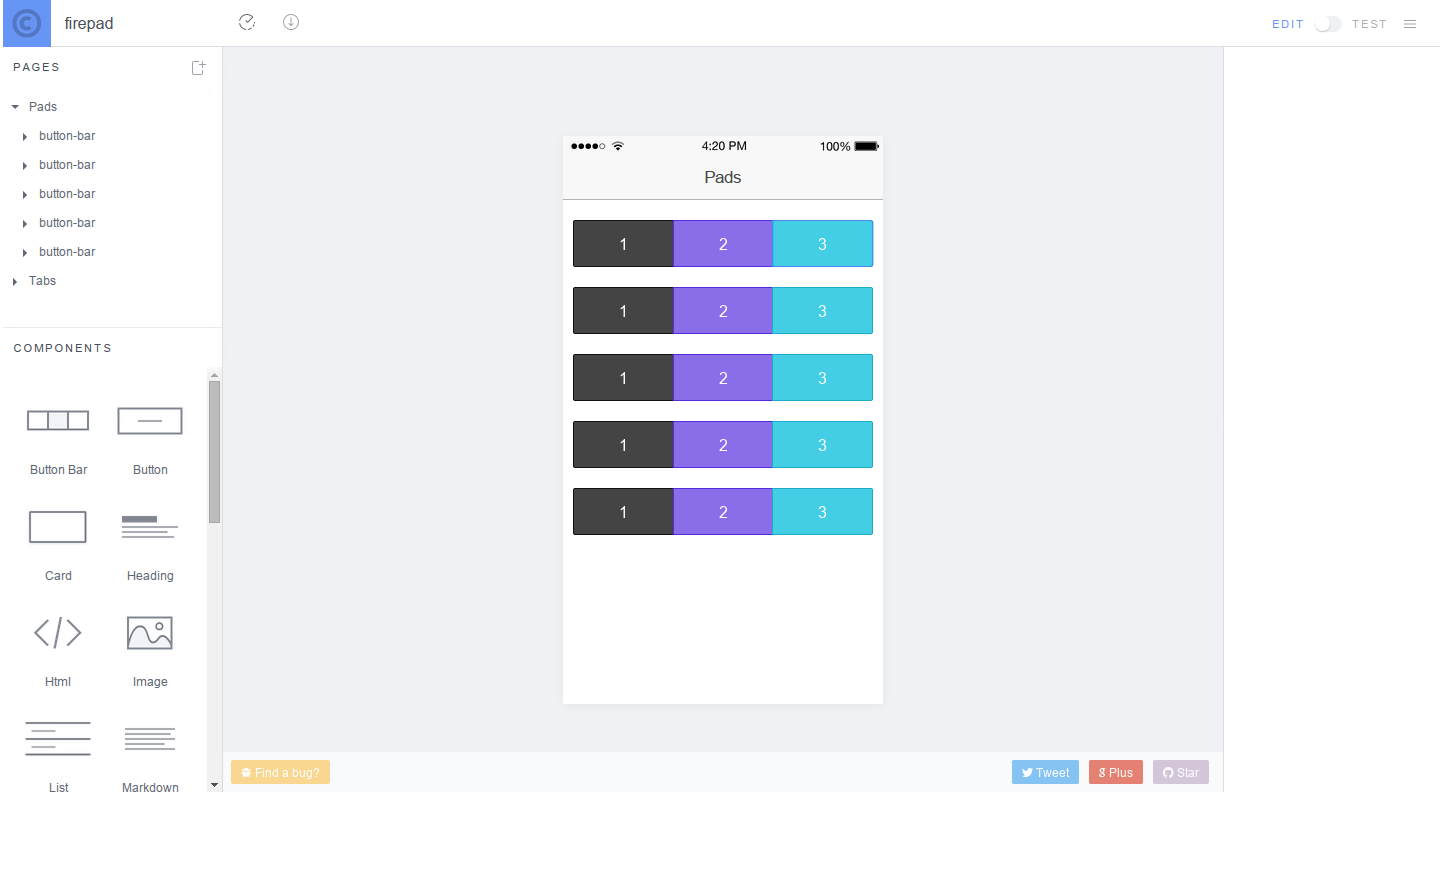
\includegraphics[scale=0.4]{Figures/ui_editor.png}
		\rule{35em}{0.5pt}
	\caption[Editor]{Editor visuale di Ionic dell'interfaccia di una applicazione}
\label{fig:Editor visuale dell'interfaccia di una applicazione}
\end{figure}


\subsection{Wrapper Framework}
il wrapper sarà il framework che ci consentirà di comunicare con le funzionalità native del dispositivo,
	-- What? --
	-- How? --
\section{La comunicazione tra le parti}
-- Tenclogia RESTFUL --\\
\subsection{Simple Rest Api}
-- Non ci occupiamo di costruire le API --\\
-- Uso delle API in angularJS --\\
-- JSON --\\
\subsection{XHR}
-- Cosè Cross Domanin --\\
-- POSTMAN --\\
-- Debug nel Browser --\\
\subsection{Firebase}
-- What, Why --\\
-- of course it's angular!! --\\
-- Ricollegarsi al discorso backend --

